% Two lineages of computing: the information utility and Unix.
% ---------------------------------------------------------------------------
% style.tex --- shared preamble for every figure in book/figures/tikz/
%
% One style for all figures: Latin Modern, thin black lines, a light grey
% fill, and one accent colour used only to mark what is untrusted or wrong.
% Build with scripts/build_figures.sh; see book/figures/README.md.
% ---------------------------------------------------------------------------
\documentclass[tikz,border=6pt]{standalone}
\usepackage[T1]{fontenc}
\usepackage{lmodern}
\usetikzlibrary{arrows.meta,positioning,shapes.geometric,calc,fit,backgrounds}

\hyphenpenalty=10000   % short lines in boxes: ragged, never hyphenated

\definecolor{lightgrey}{gray}{0.92}
\definecolor{accent}{HTML}{9B2D20}

\tikzset{
  every picture/.style={
    line width=0.6pt,
    font=\small,
    >={Stealth[length=5pt,width=4pt]},
    node distance=14pt and 24pt,
  },
  % shapes
  box/.style={draw, rectangle, inner xsep=8pt, inner ysep=5pt,
              minimum height=22pt, align=center},
  grey/.style={box, fill=lightgrey},
  rounded/.style={box, rounded corners=9pt},
  decision/.style={draw, diamond, aspect=2.4, inner sep=1.5pt, align=center},
  group/.style={draw, dashed, rounded corners=5pt, inner sep=7pt},
  % text
  tag/.style={font=\footnotesize, align=center, inner sep=2pt},
  note/.style={font=\footnotesize\itshape, align=center, inner sep=2pt},
  code/.style={font=\small\ttfamily},
  codetag/.style={font=\footnotesize\ttfamily, align=center, inner sep=2pt},
  title/.style={font=\small\scshape, align=center, inner sep=2pt},
  % lines
  arrow/.style={->},
  back/.style={->, dashed},
  thin/.style={line width=0.4pt, gray},
  % the one accent, for what is untrusted, wrong or missing
  bad/.style={accent},
  badbox/.style={box, draw=accent, text=accent},
}

\begin{document}
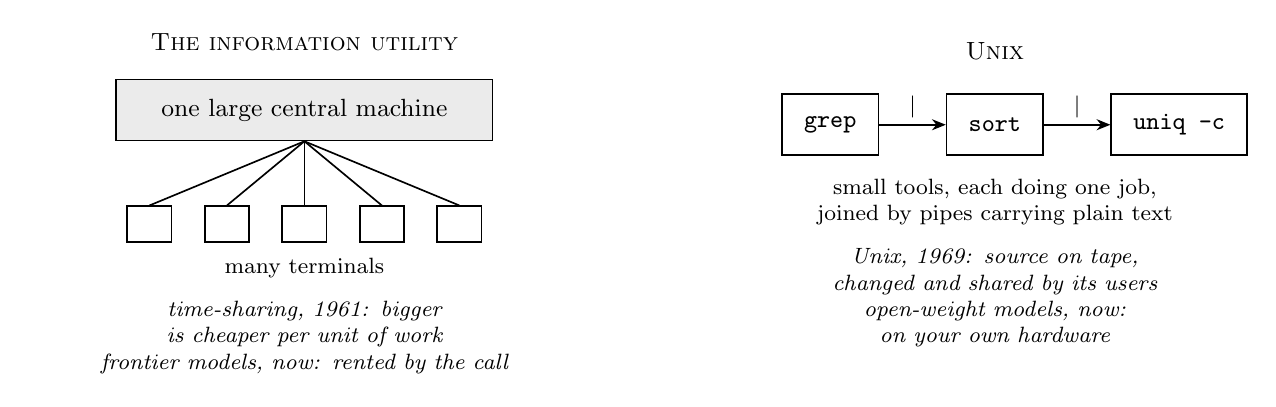
\begin{tikzpicture}
  % Left: one central plant, many terminals
  \node[title] (lt) at (0,0) {The information utility};
  \node[grey, minimum width=136pt, below=8pt of lt] (plant) {one large central machine};
  \foreach \i/\x in {1/-56,2/-28,3/0,4/28,5/56}
    \node[box, minimum width=16pt, minimum height=13pt, inner sep=1pt] (t\i)
      at ($(plant.south)+(\x pt,-30pt)$) {};
  \foreach \i in {1,...,5} \draw (plant.south) -- (t\i.north);
  \node[tag, below=3pt of t3] (term) {many terminals};
  \node[note, below=4pt of term, text width=196pt]
    {time-sharing, 1961: bigger is cheaper per unit of work\\
     frontier models, now: rented by the call};
  % Right: small tools joined by pipes
  \node[box, code] (u1) at (190pt,-30pt) {grep};
  \node[box, code, right=of u1] (u2) {sort};
  \node[box, code, right=of u2] (u3) {uniq -c};
  \node[title, above=10pt of u2] {Unix};
  \draw[->] (u1) -- node[tag, above] {\textbar} (u2);
  \draw[->] (u2) -- node[tag, above] {\textbar} (u3);
  \node[tag, below=6pt of u2] (pipes) {small tools, each doing one job,\\joined by pipes carrying plain text};
  \node[note, below=4pt of pipes, text width=176pt]
    {Unix, 1969: source on tape, changed and shared by its users\\
     open-weight models, now: on your own hardware};
\end{tikzpicture}
\end{document}
